\section{Solution}

\subsection{Overview}

We partition our system in 3 compontents (showcased in
\ref{fig:overview}):
\begin{itemize}
    \setlength{\itemsep}{0pt}
    \setlength{\parskip}{0pt}
    \setlength{\parsep}{0pt}
    \item The clients, which may or may not collaborate in a
        document;
    \item The servers, which run a fault tolerant consensus
        protocol to provide the document service;
    \item The persistent storage, which backs each server.
\end{itemize}

\begin{figure}[ht]
    \centering
    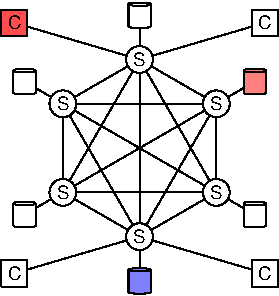
\includegraphics[width=.5\linewidth]{img/sys-1}
    \caption{System overview. Storage in blue has been rolled
    back. Storage in red has been victim of a ransomware attack.
    Client in read is malicious.}
    \label{fig:overview}
\end{figure}

\begin{table*}[ht]
    \centering
    \caption{API provided by the servers}
    \begin{tabularx}{\textwidth}{>{\hsize=.3\hsize}X | X | >{\hsize=.9\hsize}X }
        \hline
        \textbf{Function} & \textbf{Arguments} & \textbf{Result/Return} \\
        \hline
        $create$ & document name, ciphered document keys & creates the document \\
        \hline
        $add\_users$ & document name, ciphered document keys & adds collaborators  \\
        \hline
        $reset\_users$ & document name, list of signed encrypted diffs, ciphered document keys & resets the collaborators  \\
        \hline
        $add$ & document name, signed encrypted diff & new version hash \\
        \hline
        $get$ & document name & list of diffs and version hash \\
        \hline
        $compress$ & document name, signed compressed document, version hash & registers a positive ack to compressing the document\\
        \hline
        $rollback$ & document name, version hash & registers a positive ack to rollbacking a particular version\\
        \hline
    \end{tabularx}
    \label{tab:api}
\end{table*}

\subsection{Deployment}

Each server and each client will be deployed on a separate VM.
All servers communicate with each other. A client can connect to
any server.

\subsection{Secure Channels}

All communication will be ciphered using TLS. Each server will
have hardcoded the public key of an administrator. After booting,
the administrator will establish a secure channel (proving its
identity based on that public key) and provide the server with
its configuration: its private key and certificate and the list
of public keys of the other servers. For simplicity, we assume
that the set of servers is static.

Clients trust on servers is rooted on a signed certificate from a
trusted Certificate Authority. They establish a connection with a
server and verify the certificates.

The TLS library used will be \texttt{rustls}\cite{rustls}.

\subsection{Secure Protocols}

The protocol is based on the notion of applying diffs.
Clients, when editing, will periodically send the diff to a
server which will run a consensus protocol to propagate the diff
to all servers. This way, a total order of diffs is establhished,
making it possible to assign versions to the document.

Clients have asymmetric keys and are identified by their public
keys.

Diffs are signed by the author, making it possible to rollback a
diff. However, the server only rollbacks a particular diff if it
receives the requests from a majority of collaborators. This
protects against client-issued ransomware: if a client decides,
in a diff, to encrypt all the data, the rest of the clients can
simply rollback the diff.

\begin{table*}[ht]
    \centering
    \label{Effort Commitment}
    \begin{tabular}{r|l|l|l}
        & AB & BSD & WP \\
        \hline
        Nov 16th & client diffs & consensus protocol & add/get + doc creation \\
        Nov 23th & rollback & compress & document creation \\
        Nov 30th & demonstration & document membership changes & key provisioning\\
    \end{tabular}
\end{table*}

Each document has a \emph{document key}. This key is only known
to the collaborators and is used to encrypt diffs. This way, we
achieve confidentiality of the documents. Integrity is achieved
by employing the consensus protocol (which ensures that the diffs
are totally ordered, and as such the document cannot be tampered
by slightly reordering concurrent diffs) and by using an
authenticated encryption scheme (namely GCM).

The document key is chosen by the owner upon creation. To add collaborators, the owner
simply encrypts the document key with the collaborator's public
key and sends it to the servers. To remove a collaborator, the
owner has to generate a new document key, decrypt all the diffs
with the old key and re-encrypt all the diffs with the new key.
This way, the purged collaborator cannot make or see new
modifications.

It is possible to compress the document, by replacing the diff
chain with a single diff. This requires approval from a majority
of collaborators. This effectively makes it possible to remove
something from the document permanentely, if the majority agrees.
We believe this is a desirable feature, and it is the main reason
we chose this solution versus, for instance, a blockchain based
approach: if a collaborator uploads illegal/undesired content, it
can be deleted safely.

We consider that $\lfloor \frac{n - 1}{3} \rfloor$ servers can
behave in a Byzantine fashion, by having had their persistent
storage tampered with.

We refer the reader to \cite{pbft} for a description of a Byzantine
consensus protocol. In terms of the state machine (ie: the API
exposed by the servers) it is described in Table~\ref{tab:api}.

Note that in the case of the compress and rollback commands, any
client can issue the first request and the server will in its
turn ask the other clients. The clients may then either reject
the request or reply positively, making the compress and rollback
commands.

The implementation will be made in Rust\cite{rust}. There will be an
application (the server) and a client library.
